
%(BEGIN_QUESTION)
% Copyright 2011, Tony R. Kuphaldt, released under the Creative Commons Attribution License (v 1.0)
% This means you may do almost anything with this work of mine, so long as you give me proper credit

Suppose a technician opens the door of a junction box and connects a DMM (digital multimeter) to a pair of thermocouple wires landed to a terminal strip inside the box.  The thermocouple junction at the other end of this wire pair is installed in a hot process pipe about 50 feet away, measuring the temperature of a process fluid.  Noting the ambient temperature inside the junction box being 58 degrees Fahrenheit, the technician measures a thermocouple signal of 29.34 millivolts.  Calculate the temperature of this type E thermocouple.

\vskip 10pt

$T = $ \underbar{\hskip 50pt} degrees Fahrenheit

\vskip 10pt

Be sure to show your work in calculating this temperature!

\vskip 50pt

Now, suppose the technician removes the temperature transmitter connected to this type E thermocouple, taking the transmitter back to the calibration lab.  Assuming a lab room temperature of 73 degrees F and ``cold junction compensation'' activated inside this transmitter, determine the number of DC millivolts the technician would need to input to the transmitter's terminals to simulate a process (thermocouple) temperature of 925 degrees Fahrenheit.

\vskip 10pt

$V_{in} = $ \underbar{\hskip 50pt} mV

\vskip 30pt

Next, calculate the necessary resistance in this voltage divider circuit to produce this required millivoltage signal (to simulate a temperature of 925 degrees F):

$$\includegraphics[width=15.5cm]{i00629x01.eps}$$

$R = $ \underbar{\hskip 50pt} ohms



\vfil
\underbar{file i00629}
\eject
%(END_QUESTION)





%(BEGIN_ANSWER)

This is a graded question -- no answers or hints given!

%(END_ANSWER)





%(BEGIN_NOTES)

The important principle to remember here is that the voltage registered by a voltmeter or any other receiving instrument in a thermocouple circuit is always the {\it difference} between the voltages output by two series-opposed thermocouple junctions: the measurement junction and the reference junction.  The following formula expresses this fact:

$$V_{meter} = V_{J1} - V_{J2}$$

Thus, the 29.34 mV signal registered by the voltmeter in the first paragraph is actually the difference in voltage between the measurement junction (at process temperature) and the reference junction where the meter's leads connect to thermocouple wire (at 58 degrees F).  Manipulating the formula to solve for measurement junction voltage:

$$V_{J1} = V_{meter} + V_{J2}$$

Looking up the millivoltage value for a type E thermocouple at 58 $^{o}$F gives us a $V_{J2}$ value of 0.857 mV.  Adding this to our meter's registered voltage of 29.34 mV gives us a measurement junction voltage of 30.197 mV, which corresponds to a type E junction at just over 780 $^{o}$F.

\vskip 50pt

If we now take this type E thermocouple temperature transmitter to a calibration bench and subject it to a test voltage sufficient to simulate 925 degrees F, we need to ``fool'' the reference junction compensation inside the transmitter to make it ``think'' its dealing with a reference junction at room temperature (73 $^{o}$F).  Once again, our basic thermocouple formula tells us that the voltage typically seen by this instrument while the process temperature is 925 $^{o}$F and the terminal temperature is 73 $^{o}$F will be the {\it difference} between those corresponding voltages.  Looking up the voltage values for a type E thermocouple at 925 $^{o}$F and 73 $^{o}$F gives us numbers to plug into this equation:

$$V_{meter} = V_{J1} - V_{J2}$$

$$V_{meter} = 36.691 \hbox{ mV} - 1.360 \hbox{ mV}$$

$$V_{meter} = 35.331 \hbox{ mV}$$

The resistor value necessary to generate this much voltage drop may be found by using the voltage divider formula:

$$35.331 \hbox{ mV} = 1.25 \left( {4700 \over R + 4700} \right)$$

$$R = 161.585 \hbox{ k}\Omega$$

%INDEX% Measurement, temperature: thermocouple

%(END_NOTES)


